\chapter{Web Service Security}
\begin{itemize}
	\item \textbf{Frühe Architektur: Die Insel}: Daten und Applikationen bleiben lokal und werden dort geschützt.
	\item \textbf{Später: Burgarchitektur:} Applikationen bleiben lokal, \enquote{Burgen} sind vernetzt, Daten müssen auch auf dem Transport geschützt werden
	\item \textbf{Heute: Cloudarchitektur:} Daten und Applikationen können überall sein. Daten müssen unabhängig vom Ort geschützt werden.
\end{itemize}
\begin{figure}[H]
	\begin{center}
		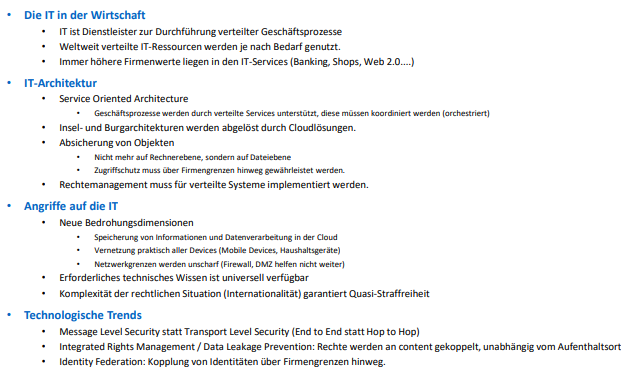
\includegraphics[scale=0.8]{Resources/itsicherheit}
		\caption{}
		\label{fig:itsicherheit}
	\end{center}
\end{figure}

\paragraph{Folgen dieser Entwicklungen:}
\begin{itemize}
	\item \textbf{Unscharfe Netzwerkgrenzen:} \textbf{klassischer Permimeterschutz} versagt zunehmend
	\item Umgehung von Sicherheitsmechanismen zunehmend leichter für Nutzer (Dropbox statt firmeneigener Dateiablage, etc.)
\end{itemize}
$\Rightarrow$ Sicherheit auf Kommunikationswegen muss ergänzt werden um Mechanismen, welche Daten überall schützen.\\
$\Rightarrow$ Produktivitätseinschränkende Sicherheitsmechanismen laufen ins Leere!

\section{SSO über Trust Domänen hinweg}
\begin{figure}[H]
	\begin{center}
		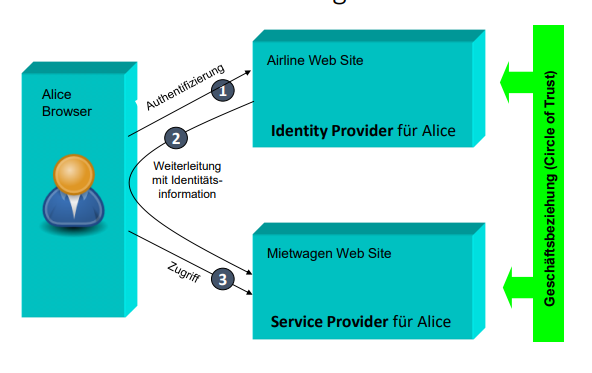
\includegraphics[scale=0.8]{Resources/SSO}
		\caption{}
		\label{fig:SSO}
	\end{center}
\end{figure}

\section{Federated Identity: Account Linking}
\begin{figure}[H]
	\begin{center}
		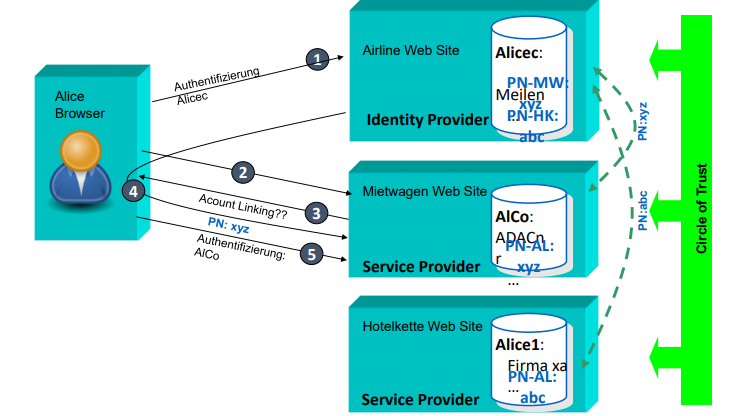
\includegraphics[scale=0.8]{Resources/FedIdent1}
		\caption{Account Linking}
		\label{fig:FedIden1}
	\end{center}
\end{figure}
\begin{figure}[H]
	\begin{center}
		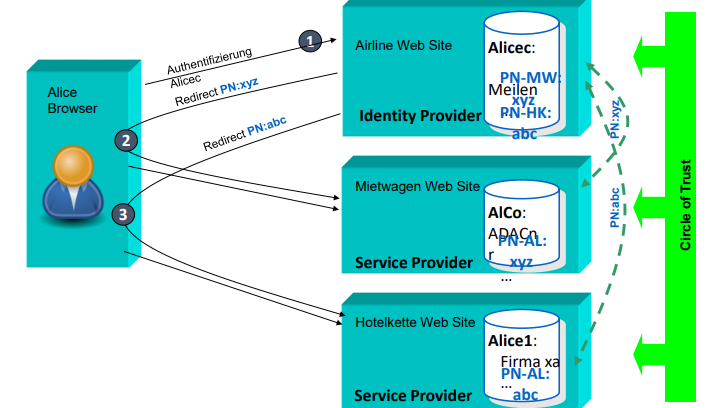
\includegraphics[scale=0.8]{Resources/FedIden2}
		\caption{nach dem Linken}
		\label{fig:FedIden2}
	\end{center}
\end{figure}

\section{XML - Signaturen}
\begin{figure}[H]
	\begin{center}
		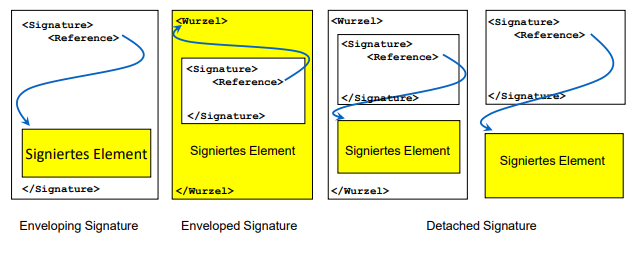
\includegraphics[scale=0.8]{Resources/XMLSig}
		\caption{}
		\label{fig:XMLSig}
	\end{center}
\end{figure}

\subsection{XML-Signatur - Enveloped Signature}
\begin{figure}[H]
	\begin{center}
		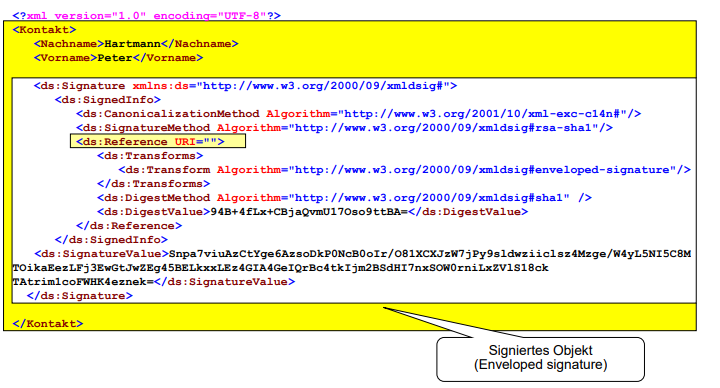
\includegraphics[scale=0.8]{Resources/EnvelopedSignature}
		\caption{}
		\label{fig:EvelopedSignature}
	\end{center}
\end{figure}

\subsection{XML-Signatur - Enveloping Signature}
\begin{figure}[H]
	\begin{center}
		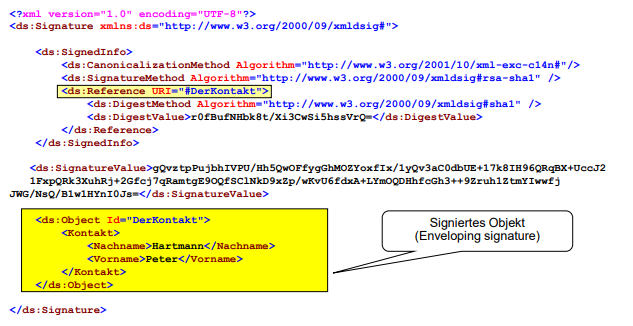
\includegraphics[scale=0.8]{Resources/EnvelopingSignature}
		\caption{}
		\label{fig:EvelopingSignature}
	\end{center}
\end{figure}

\subsection{XML-Signatur - Detached Signature}
\begin{figure}[H]
	\begin{center}
		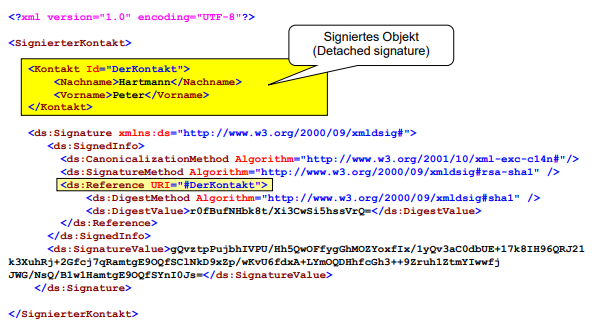
\includegraphics[scale=0.8]{Resources/DetachedSignature}
		\caption{}
		\label{fig:DetachedSignature}
	\end{center}
\end{figure}

\subsection{XML-Signatur - Detached Signature2}
\begin{figure}[H]
	\begin{center}
		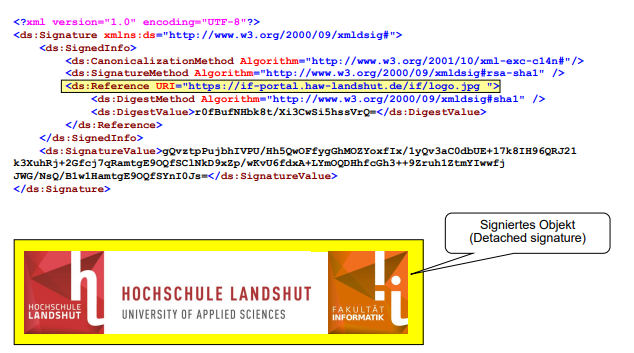
\includegraphics[scale=0.8]{Resources/DetachedSignature2}
		\caption{}
		\label{fig:DetachedSignature2}
	\end{center}
\end{figure}

\section{XML-Encryption}
\subsection{Klartextnachricht}
\begin{figure}[H]
	\begin{center}
		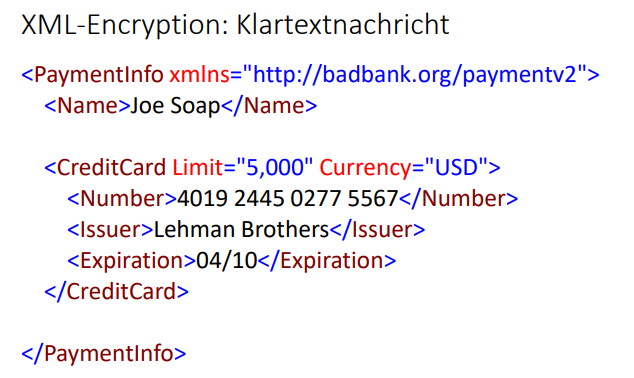
\includegraphics[scale=0.8]{Resources/XMLEncrypt1}
		\caption{}
		\label{fig:XMLEncrypt1}
	\end{center}
\end{figure}

\subsection{encrypted Element}
\begin{figure}[H]
	\begin{center}
		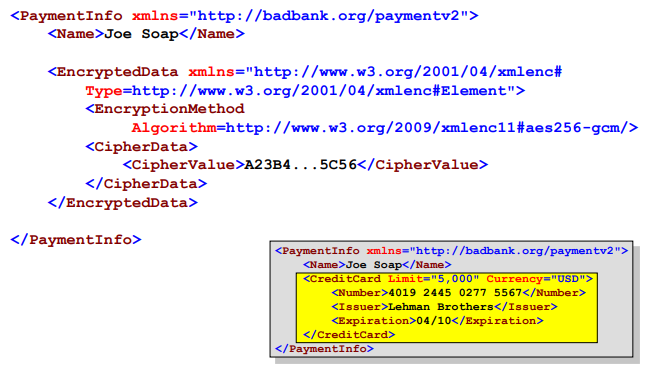
\includegraphics[scale=0.8]{Resources/XmlEncrypt2}
		\caption{}
		\label{fig:XmlEncrypt2}
	\end{center}
\end{figure}

\subsection{encrypted contnent}
\begin{figure}[H]
	\begin{center}
		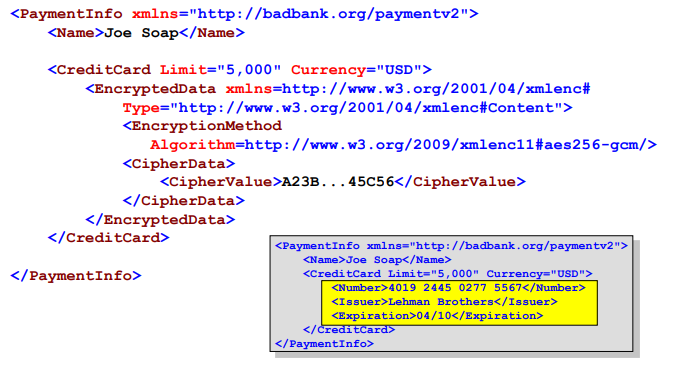
\includegraphics[scale=0.8]{Resources/XmlEncrypt3}
		\caption{}
		\label{fig:XmlEncrypt3}
	\end{center}
\end{figure}

\subsection{KeyInfo in EncryptedData}
\begin{figure}[H]
	\begin{center}
		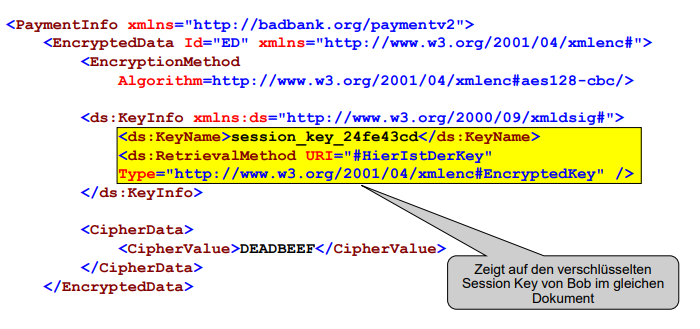
\includegraphics[scale=0.8]{Resources/XmlEncrypt4}
		\caption{}
		\label{fig:XmlEncrypt4}
	\end{center}
\end{figure}

\section{Verschlüsseln und Signieren}
\paragraph{Encrypt-Sign}
\begin{itemize}
	\item Trudy kann abhören und die Signatur austauschen
	\item \textbf{Abhilfe:} Vor dem Verschlüsseln in den Klartext den Absendernamen schreiben.
\end{itemize}

\paragraph{Sign-Encrypt}
\begin{itemize}
	\item Der vorgesehene Empfänger kann die Nachricht um-verschlüsseln und weiterleiten
	\item der falsche Empfänger denkt die Nachricht ist für ihn
	\item \textbf{Abhilfe:} Alice kann vor dem Signieren den Klartext in den Empfängernamen schreiben
\end{itemize}

\section{SAML-assertions}










